\chapter{Feature Selection}
\label{ch:feature-selection}
\index{Feature Selection|(}

\textit{Feature Selection} (FS) is a process that chooses an optimal subset of features according to certain criterion \citep{liu2012feature}. According to \citet{sammut2017encyclopedia}, in many real-world applications, such as data mining, machine learning, computer vision, and bioinformatics, we need to deal with high-dimensional data. Lately, the dimensionality of the data involved in these areas has increased exponentially. The trend of this growth of the \textit{UCI machine learning repository}\footnote{https://archive.ics.uci.edu/ml/index.php} is shown in Figure~\ref{fig:fs_growth}.

\begin{figure}
  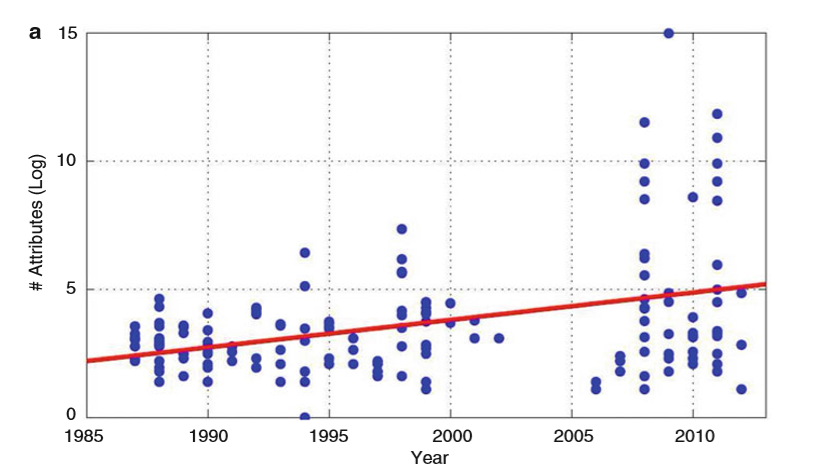
\includegraphics{feature_selection/growth.png}
  \caption{Growth of the number of features in the UCI ML repository. Reproduced from \citet{sammut2017encyclopedia}.}
  \label{fig:fs_growth}
\end{figure}

\citet{guyon2003introduction} state that the objective of FS is three-fold: improving the prediction performance of the predictors, providing faster and more cost-effective predictors, and providing a better understanding of the underlying process that generated the data. Furthermore, the aim the FS is to select features that are \textit{independent} of each other but \textit{highly dependent} on the value to be predicted.

FS keeps the original feature, that is, it maintains the physical meanings of the original feature without any transformation. Furthermore, \citet{masaeli2010transformation} found that this property has its significance in many practical applications such as finding relevant genes to a specific disease and building a sentiment lexicon for sentiment analysis.

According to \citet{zhao2010advancing}, FS is an optimization problem that can be split into two perspective; (1) searching for the best subset of features, (2) principle model for selecting, adding removing or changing new features during the search using a certain evaluation measure. Mainly there are three models used for FS: filter, wrapper and embedded.

\section{Filter Models}\label{sec:fs_filter}\index{Feature Selection!filter models}
\textit{Filter models} operate independently of the learning algorithm. A filter algorithm usually consists of two steps. First, each feature is given a weight then, the features are ranked and the top-ranking features are chosen whilst the others are discarded. Some popular measurements use to calculate feature weight are; distance measures, information measures, dependency measures, and consistency measures.

\begin{itemize}
  \item \textit{Distance measure}\index{Feature Selection!distance measure}: is also known as separability, divergence, or discrimination measure. When using distance measure for a two-class problem to choose a feature, the feature may be chosen or discarded as shown in the following example: feature $f_{1}$ is preferred to feature $f_{2}$ if $f_{1}$ induces a greater difference between the two-class conditional probabilities than $f_{2}$, because we try to find the feature that can separate the two classes as far as possible. $f_{1}$ and $f_{2}$ are indistinguishable if the difference is zero \citep{liu2005toward}. \citet{de2015feature} state that two popular distance measures used in FS are \textit{directed divergence} and \textit{variance}.
  \item \textit{Information measure}\index{Feature Selection!information measure}: typically determines the information gain from a feature. The information gain from a feature, example $f_{1}$, is defined as the difference between the prior uncertainty and expected posterior uncertainty using $f_{1}$. Feature $f_{1}$ is preferred to feature $f_{2}$ if the information gain from $f_{1}$ is greater than that from $f_{2}$ \citep{liu2005toward}. A commonly used information measure function is \textit{Shannon`s entropy} \citep{de2015feature}.
  \item \textit{Dependency measure}\index{Feature Selection!dependency measure}: is also known as correlation measure or similarity measure. It measures the ability to predict the value of one variable from the value of another. In FS for classification, we look for how strongly a feature is associated with the class. A feature $f_{1}$ is preferred to another feature $f_{2}$ if the association between feature $f_{1}$ and class $C$ is higher than the association between $f_{2}$ and $C$. In FS for clustering, the association between two random features measures the similarity between the two \citep{liu2005toward}. Two common dependency measure functions are \textit{Pearson's correlation} and \textit{Bhattacharyya dependence} \citep{de2015feature}.
  \item \textit{Consistency measure}\index{Feature Selection!consistency measure}: This type of evaluation measure is characteristically different from other measures because of it's heavy reliance on the training dataset and use of Min-Features bias in selecting a subset of features. Min-Features bias prefers consistent hypotheses definable over as few features as possible. This measure finds out the minimal size subset that satisfies the acceptable inconsistency rate, that is usually set by the user \citep{liu2005toward}.
\end{itemize}

Filter models normally are very fast because usually the evaluation measurement complexity is simple and cheap, both in terms of performance and memory. Having said this, \citet{garcia2015data} found that due to it's simplicity and low time complexity it can handle large data. On the other hand, \citet{guyon2003introduction} found that due to the fact that filter models score features independently of each other, the best features are not always chosen. This is because, a feature that is completely useless by itself thus ranked very low with this model, can provide a significant performance improvement when taken with others. \textit{Wrapper models} address this limitation by evaluating subsets of features rather than individual features.

\section{Wrapper Models}\label{sec:fs_filter}\index{Feature Selection!wrapper models}
The aim of the \textit{Wrapper model} is to achieve the highest predictive accuracy possible by selecting the features that accomplish this for a fixed learning algorithm. It uses a learning algorithm as a black-box to select the best feature subset, agreeing on a predictive measure \citep{kohavi1995study}. Figure \ref{fig:fs_wrapper} shows a conceptual view of a wrapper model. The \textit{Feature Selector} component takes on the original features and uses a search strategy to generate subsets of features for evaluation. The selected feature subset uses the learning algorithm to \textit{measure} and evaluate its performance. These steps are repeated until a \textit{stopping criterion} is met. Typically, the stopping criterion is that refinements to the subset do not yield any performance improvements.

\begin{figure}
  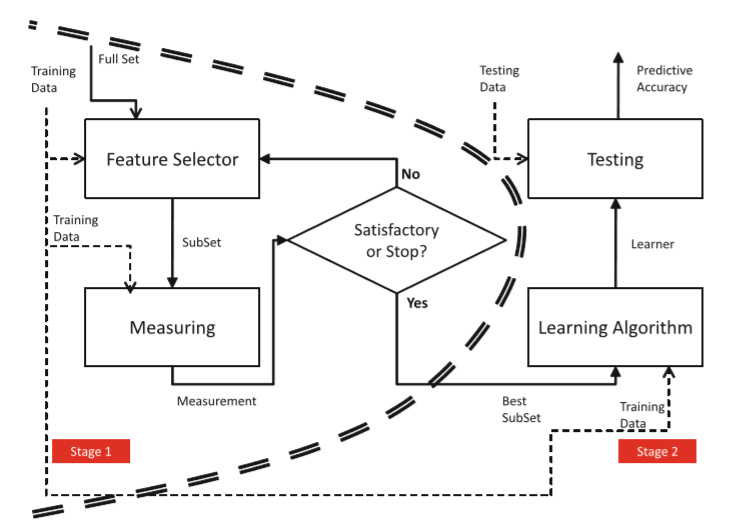
\includegraphics{feature_selection/wrapper.png}
  \caption{A general framework for Wrapper Methods of FS. Reproduced from \citet{tang2014feature}}
  \label{fig:fs_wrapper}
\end{figure}

Since there are a lot of ways and combinations on how to select the feature set, feature search plays an important role in wrappers model. One can classify feature search strategies into; Exponential search, Sequential search and Randomized search \citep{de2015feature}.

\begin{itemize}
  \item\textbf{Exponential search}\index{Feature Selection!exponential search}: An exponential search returns the optimal subset. Although the order of the search space is $O(2^N)$, the search need not be exhaustive, i.e. heuristics can be introduced to reduce the search space without compromising the chances of discovering the optimal subset \citep{liu2005toward}.
  \item\textbf{Sequential search}\index{Feature Selection!sequential search}: Sequential forward feature selection (SFFS), sequential backward feature elimination (SBFE) and bidirectional selection are greedy search algorithms that add or remove features one at a time \citep{liu2005toward}. SFFS initiates with an empty set and SBFE initiates with a full set where as a bidirectional search initiates a SFFS and SBFE simultaneously ensuring that the features selected by SFFS are never eliminated by SBFE.
  \item\textbf{Randomized search}\index{Feature Selection!randomized search}: In practical applications, the feature space may contain thousands of features. In such applications, it is not feasible to search the entire feature space. Randomized search trades off optimality of the solution for efficiency by searching only a sampled portion of the feature space. Genetic Algorithms have been used as a guided randomized FS technique \citep{cherkauer1996growing, vafaie1995genetic}.
\end{itemize}

According to \citet{sammut2017encyclopedia}, wrapper models generally achieve better recognition rates than filter models since the learning algorithm is involved in the selection of the subset, thus any bias introduced by the chosen algorithm is removed. The drawback of this model is that, wrapper models must train a classifier for each feature subset thus the method might become unfeasible.

\section{Embedded models}\label{sec:fs_filter}\index{Feature Selection!embedded models}
Some learning algorithms have in-built mechanisms to deal with feature selection \citep{guyon2003introduction,sammut2017encyclopedia}. This makes the selection of the features more efficient than the wrapper method and is specifically designed for the algorithm of choice. Another improvement on the other methods is that whilst the filter and wrapper methods select the features as part of the pre-processing of the data, the embedded models cater for feature selection as part of the learning process. One such example is the use of \textit{L1-norm} regularisation in \textit{Support Vector Machines} (SVM) \citep{guyon2003introduction,de2015feature}. Here the coefficients of less important features are reduced to zeros thus eliminating them. \textit{L2-norm} regularisation can also be used for feature selection but was found to be less effective than \textit{l1-norm} regularisation \citep{de2015feature}. \textit{Decision trees} also have a feature selection strategy embedded within the algorithm \citep{garcia2015data}.

\index{Feature Selection|)}